\documentclass[final]{article}

\usepackage{aps360}
\usepackage[utf8]{inputenc}
\usepackage[T1]{fontenc}
\usepackage{hyperref}
\usepackage{url}
\usepackage{booktabs}
\usepackage{amsmath}
\usepackage{amssymb}
\usepackage{microtype}
\usepackage{graphicx}
\graphicspath{{image/}}
\usepackage{tikz}
\usetikzlibrary{arrows.meta, positioning, calc}

% Reduce space between section headers and body text
\makeatletter
\renewcommand{\section}{%
  \@startsection{section}{1}{\z@}%
                {-1.5ex \@plus -0.3ex \@minus -0.2ex}%
                {0.4ex \@plus 0.1ex}%
                {\large\bf\raggedright}%
}
\makeatother

% Slightly tighten inter-paragraph spacing to keep the main text within 3 pages
\setlength{\parskip}{4.5pt}

% Override geometry: tighter top/bottom margins
\AtBeginDocument{%
  \newgeometry{%
    textheight=9.5in,
    textwidth=5.5in,
    top=0.65in,
    headheight=12pt,
    headsep=15pt,
    footskip=18pt%
  }%
}

\title{Pose-Based Human Action Recognition for Athletic Movement Analysis\\\large Progress Report}
\author{%
  Harry Zhang\\
  1010988843, harryh.zhang@mail.utoronto.ca\\
  https://github.com/po8onthetrack/Deep-Learning-Project\\
}

\begin{document}

\maketitle
\vspace{-0.45in}

\section*{Brief Project Description}
This project is motivated by the author's experience with badminton and bouldering, where reading how the body moves is the first step toward better technique and fewer injuries. The goal is markerless action recognition from body pose alone: given a short sequence of 17 body-keypoint positions tracked across video frames from a single camera (the \textbf{input}), classify it into one of the 20 MPOSE2021 action categories (the \textbf{output}). Deep learning is appropriate because an action is defined by \emph{how} the joints move over time --- a spatio-temporal pattern that cannot be captured by a fixed rule over keypoints; a recurrent network learns both the pose configuration in each frame and its dynamics across frames \citep{du2015hierarchical}. Reliable markerless action recognition is a building block for downstream movement analysis, training feedback, and injury-aware coaching.\footnote{Portions of the writing and code in this project were developed with the assistance of Claude \citep{anthropic2026claude} and Claude Code \citep{anthropic2026claudecode}.}

\begin{figure}[!h]
\centering
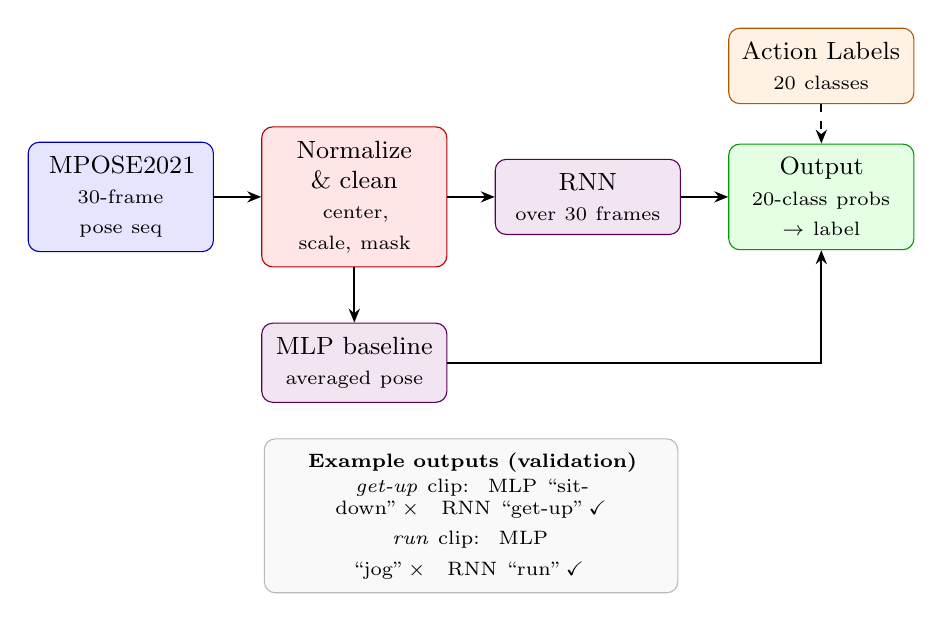
\begin{tikzpicture}[
  node distance=0.5cm and 0.6cm,
  box/.style={rectangle, rounded corners=4pt, align=center, font=\small,
              minimum height=0.9cm, text width=2.0cm, inner sep=5pt},
  arr/.style={-{Stealth[length=5pt, width=4pt]}, thick}
]
\node[box, draw=blue!70!black,   fill=blue!10]     (mpose)
  {MPOSE2021\\\scriptsize 30-frame pose seq};
\node[box, draw=red!70!black,    fill=red!10,      right=0.6cm of mpose] (prep)
  {Normalize \& clean\\\scriptsize center, scale, mask};
\node[box, draw=violet!70!black, fill=violet!10,   right=0.6cm of prep] (rnn)
  {RNN\\\scriptsize over 30 frames};
\node[box, draw=green!60!black,  fill=green!10,    right=0.6cm of rnn] (eval)
  {Output\\\scriptsize 20-class probs $\to$ label};
\node[box, draw=violet!70!black, fill=violet!10,   below=0.7cm of prep] (mlp)
  {MLP baseline\\\scriptsize averaged pose};
\node[box, draw=orange!70!black, fill=orange!10,   above=0.5cm of eval] (labels)
  {Action Labels\\\scriptsize 20 classes};
\draw[arr] (mpose) -- (prep);
\draw[arr] (prep)  -- (rnn);
\draw[arr] (rnn)   -- (eval);
\draw[arr] (prep)  -- (mlp);
\draw[arr] (mlp.east) -| (eval.south);
\draw[arr, dashed] (labels) -- (eval);
\coordinate (cx) at ($(mpose)!0.5!(eval)$);
\node[box, draw=gray!55, fill=gray!5, text width=4.9cm, anchor=north] (ex)
  at ([yshift=-0.45cm]cx |- mlp.south)
  {\scriptsize\textbf{Example outputs (validation)}\\[1pt]
   \scriptsize\emph{get-up} clip:\; MLP ``sit-down''\,$\times$\quad RNN ``get-up''\,$\checkmark$\\
   \scriptsize\emph{run} clip:\; MLP ``jog''\,$\times$\quad RNN ``run''\,$\checkmark$};
\end{tikzpicture}
\caption{Pipeline. \textbf{Input:} a 30-frame sequence of 17 body keypoints $(x,y,\mathrm{conf})$, normalised and cleaned. \textbf{Output:} a probability distribution over the 20 action classes; the class with the highest probability is reported as the predicted action label, scored against the ground-truth labels (dashed) with accuracy and macro-F1. The grey box lists actual validation predictions (cf.\ Figures~\ref{fig:baseline}--\ref{fig:primary}): the static MLP baseline confuses motion-dependent pairs that the temporal RNN resolves.}
\label{fig:pipeline}
\end{figure}

\section*{Data Processing}
\textbf{Source and statistics.} MPOSE2021 \citep{mazzia2021action,mpose2021zenodo,pic4ser2021mpose} provides 30-frame clips of 17 COCO keypoints, shape \texttt{(30,17,3)} as $(x,y,\mathrm{conf})$, each with a human-annotated label over 20 action classes. The \emph{PoseNet} keypoints are used, as their 17-joint COCO format matches the MoveNet front-end used at deployment, so no remapping is needed. The set has \textbf{15{,}429} clips; the official cross-subject split~1 gives \textbf{12{,}562} train and \textbf{2{,}867} test.

\textbf{Cleaning (reproducible).} Each frame is (1)~\emph{normalised} --- centred at the mid-hip and scaled by torso length (mid-hip to mid-shoulder) --- to remove body size, camera distance, and screen position, as the raw coordinates are pixels, not normalised; (2)~\emph{cleaned} --- joints with confidence $<0.2$ have their $(x,y,\mathrm{conf})$ zeroed, so undetected joints (which arrive at $(0,0)$) are flagged rather than entered as real positions; and (3)~\emph{flattened} to per-frame 51-vectors, giving sequences of shape \texttt{(N,30,51)}. Inverse-frequency class weights from the training labels feed a weighted cross-entropy loss to counter imbalance.

\textbf{Split.} The official cross-subject test set is held out and scored once; a validation set is carved from train by stratified sampling, giving \textbf{train 10{,}351 / val 2{,}211 / test 2{,}867} ($\approx$67/14/19\%).

\begin{figure}[!h]
\centering
\sbox0{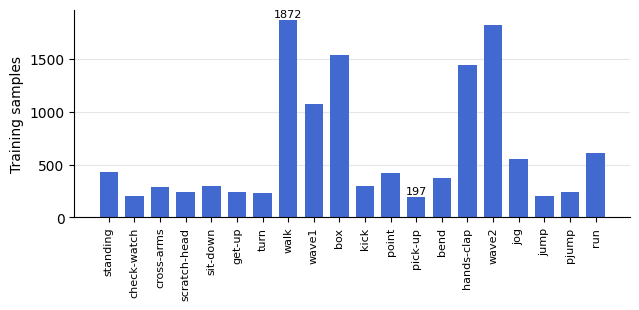
\includegraphics[width=0.5\linewidth]{class_distribution.png}}%
\usebox0\hfill
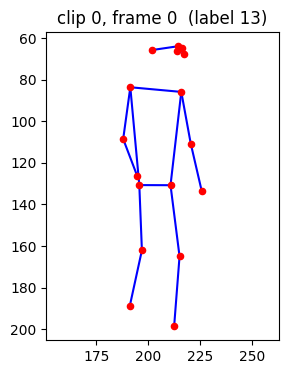
\includegraphics[height=\ht0]{cleaned_sample.png}
\caption{Left: class distribution is heavily imbalanced --- the largest class (1{,}872 samples, 14.9\%) outnumbers the smallest (197, 1.6\%) by $\approx$9.5$\times$, motivating the weighted loss and the use of macro-F1. Right: an example cleaned, hip-centred, torso-scaled skeleton.}
\label{fig:data}
\end{figure}

\textbf{New-data test plan.} For final testing on unseen data, the author will record $\approx$5 takes each of $\approx$10--12 feasible actions ($\approx$50--60 short clips; static camera, full body in frame, position and speed varied between takes), extract keypoints with frozen MoveNet \citep{tensorflowmovenet}, apply the identical pipeline, and evaluate the trained model exactly once --- these clips are never used for training or tuning. The same setup doubles as the real-time demo.

\textbf{Challenges.} The dominant difficulty was the severe class imbalance: with an unweighted loss, a model can score well by favouring frequent classes and neglecting rare ones. Inverse-frequency class weights $w_c = N/(K\,n_c)$ ($N$ training samples, $K{=}20$ classes, $n_c$ count of class $c$) are therefore passed to the cross-entropy loss, making a rare-class mistake cost proportionally more; the computed weights span 0.34--3.19, and macro-F1 is the headline metric so residual neglect stays visible. A second difficulty, noisy occluded keypoints, is handled by the confidence-gated cleaning above.

\section*{Baseline Model}
Two reference points are used. A \textbf{majority-class predictor} (always predict the most frequent action) gives a trivial lower bound. The reported baseline is an \textbf{averaged-pose MLP}: the 30 frames are averaged into a single 51-dim pose vector, then classified by \texttt{Linear(51,128)} $\to$ ReLU $\to$ Dropout$(0.5)$ $\to$ \texttt{Linear(128,64)} $\to$ ReLU $\to$ Dropout$(0.5)$ $\to$ \texttt{Linear(64,20)} ($\approx$16K parameters). It is trained with weighted cross-entropy, Adam (lr~$10^{-3}$), and early stopping on validation macro-F1. The baseline uses the \emph{same} keypoint input as the primary model but discards all temporal information, so comparing the RNN against it isolates the value of temporal dynamics.

\begin{table}[!h]
\centering\small
\begin{tabular}{lcc}
\toprule
Model & Accuracy & Macro-F1 \\
\midrule
Majority-class (lower bound) & 0.15 & 0.01 \\
Averaged-pose MLP (baseline) & 0.63 & 0.56 \\
\midrule
RNN (primary model, 2-layer LSTM) & \textbf{0.87} & \textbf{0.82} \\
\bottomrule
\end{tabular}
\caption{Validation performance. The averaged-pose MLP lifts macro-F1 from $\approx$0.01 (majority lower bound) to 0.56, and the temporal RNN reaches 0.82 --- a further $+0.26$ that isolates the value of modelling motion over time.}
\label{tab:results}
\end{table}

\textbf{Quantitative result.} The MLP reaches $\approx$0.63 accuracy and $\approx$0.56 macro-F1 on validation (Table~\ref{tab:results}), far above the majority lower bound. The learning curves (Figure~\ref{fig:baseline}, left) show both losses decreasing together, validation below training --- expected under dropout --- so the model is not overfitting.

\textbf{Qualitative result.} The validation confusion matrix (Figure~\ref{fig:baseline}, right) is strongly diagonal but shows systematic errors with one common cause: actions whose \emph{time-averaged} pose is nearly identical but whose \emph{motion} differs. The two clearest are the temporal-reverse pair \textbf{get-up}/\textbf{sit-down} (64\% of get-up predicted as sit-down, since averaging erases the direction of motion) and the speed pair \textbf{run}/\textbf{jog} (41\%) --- distinctions that live in \emph{how} the pose evolves, which a single averaged frame cannot capture and the recurrent model is built to recover.

\begin{figure}[!h]
\centering
\sbox0{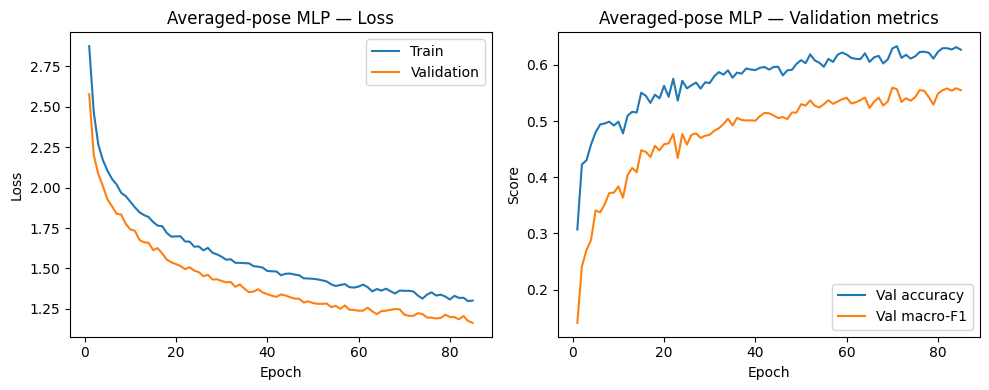
\includegraphics[width=0.44\linewidth]{mlp_curves.png}}%
\usebox0\hfill
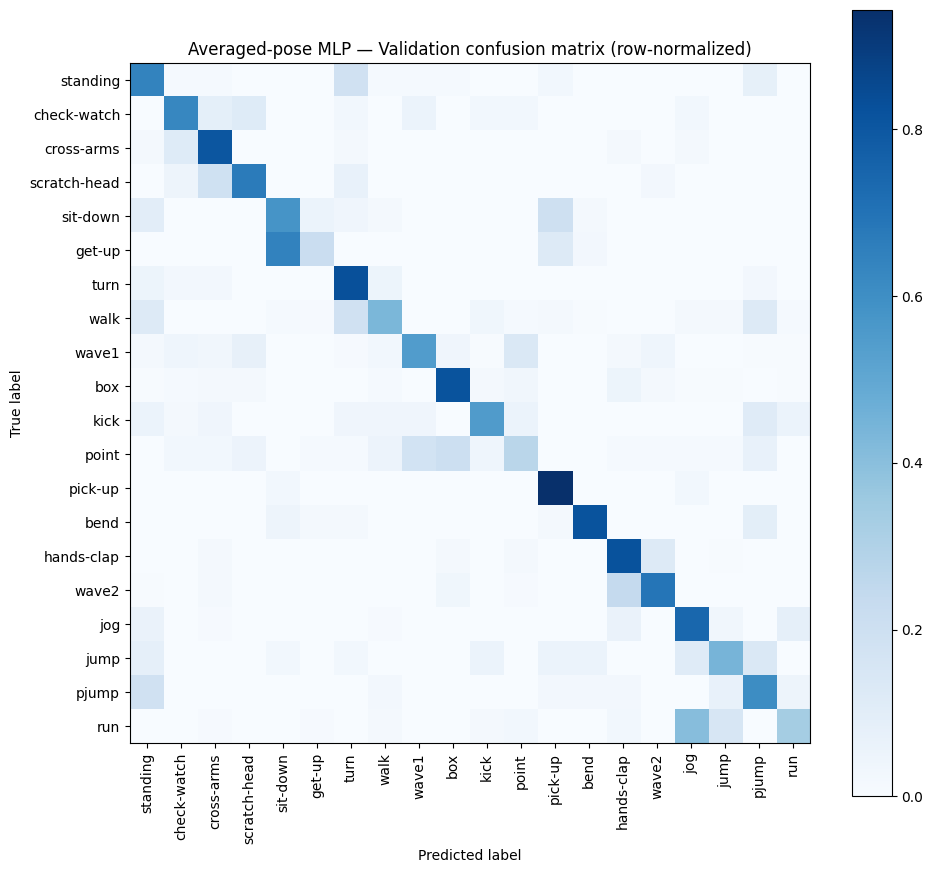
\includegraphics[height=\ht0]{mlp_confusion.png}
\caption{Averaged-pose MLP baseline. Left: learning curves. Right: row-normalised confusion matrix showing which actions are confused when temporal information is discarded.}
\label{fig:baseline}
\end{figure}

\textbf{Challenges.} Early runs collapsed onto the most frequent classes, corrected by the weighted loss (Data Processing). Frame-averaging is a deliberate limitation: it removes the temporal signal so the comparison with the RNN is controlled.

\section*{Primary Model}
\textbf{Architecture.} The primary model is a recurrent network that reads the pose sequence in temporal order: a \textbf{two-layer} LSTM (input 51, hidden 128 per layer, \texttt{batch\_first}, dropout 0.3 between the recurrent layers) processes the 30 frames, and the top layer's final hidden state --- a summary of the whole motion --- passes through Dropout$(0.3)$ and a \texttt{Linear(128,20)} layer to produce the class logits ($\approx$227K parameters, vs.\ $\approx$16K for the MLP). This is a many-to-one design (30 frames in, one label out); LSTM gates are chosen over a plain RNN to retain information across the full 30-frame window.

\textbf{Training.} The protocol is identical to the baseline for a fair comparison: weighted cross-entropy, Adam (lr~$10^{-3}$), dropout, and early stopping on validation macro-F1, which halted at epoch~82 and restored the best (epoch-67) weights. For reproducibility: seed 66, batch size 64 (train) / 256 (eval), 100-epoch cap, patience 15.

\textbf{Quantitative result.} The two-layer RNN reaches \textbf{0.87} validation accuracy and \textbf{0.82} macro-F1 (Table~\ref{tab:results}, Figure~\ref{fig:primary}), a large gain over the averaged-pose MLP ($0.63$ / $0.56$) --- a $+0.26$ macro-F1 improvement. A single-layer ablation trained under the identical protocol reaches $0.84$ / $0.77$, so the second recurrent layer alone contributes $+0.046$ macro-F1. This confirms the project's central hypothesis: modelling \emph{how} the pose evolves over time, rather than a single averaged pose, is worth the added complexity.

\textbf{Qualitative result.} The confusion matrix (Figure~\ref{fig:primary}) shows the RNN resolving precisely the motion-dependent errors that dominated the baseline: the temporal-reverse pair \textbf{get-up}/\textbf{sit-down} collapses from \textbf{0.64} (MLP) to \textbf{0.21} once the model can read the \emph{direction} of motion, and the speed-based \textbf{run}/\textbf{jog} confusion falls from 0.41 to 0.11. Every remaining error is $\le$0.21; the largest outside the reverse pair, \textbf{point}$\,\to\,$\textbf{wave1} (0.18), is an ambiguity between two single-arm gestures with similar trajectories.

\begin{figure}[!h]
\centering
\sbox0{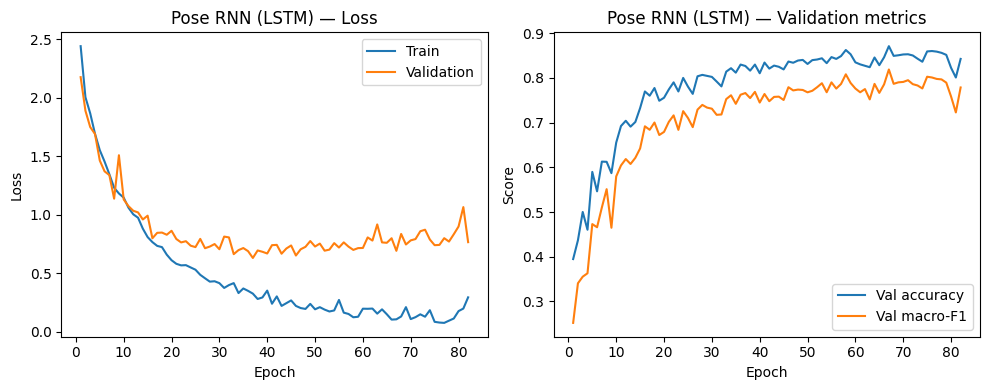
\includegraphics[width=0.44\linewidth]{rnn_curves.png}}%
\usebox0\hfill
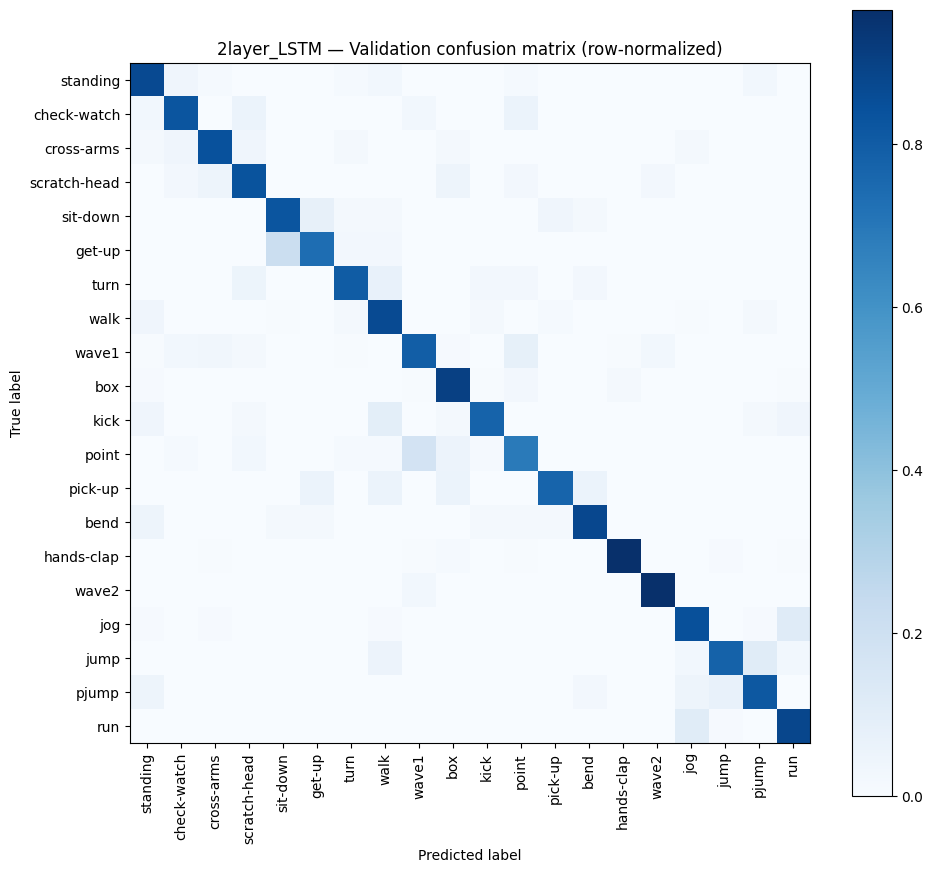
\includegraphics[height=\ht0]{rnn_confusion.png}
\caption{Primary two-layer RNN. Left: learning curves. Right: row-normalised confusion matrix; the motion-dependent confusions from the baseline (get-up/sit-down, run/jog) are largely resolved.}
\label{fig:primary}
\end{figure}

\textbf{Challenges.} Since recurrent architectures had not yet been covered in the course when the LSTM was selected for this task, a substantial share of the effort went into self-directed study of recurrent networks --- their structure, gating mechanism, and training behaviour. Training loss also fell well below validation loss in later epochs (mild overfitting); dropout and early stopping on macro-F1 kept the reported model at its best-generalising point. Systematic one-change-at-a-time tuning promoted the second recurrent layer ($+0.046$ macro-F1); weight decay and a wider hidden state (256) did not improve on it, and bidirectional/GRU variants remain for the final report.

\newpage
\begin{thebibliography}{9}

\bibitem[Anthropic(n.d.a)]{anthropic2026claude}
Anthropic. (n.d.).
\newblock Claude.ai.
\newblock \url{https://claude.ai}. Accessed June 2, 2026.

\bibitem[Anthropic(n.d.b)]{anthropic2026claudecode}
Anthropic. (n.d.).
\newblock Claude Code.
\newblock \url{https://www.anthropic.com/claude-code}. Accessed June 2, 2026.

\bibitem[Bazarevsky et~al.(2020)]{bazarevsky2020blazepose}
Bazarevsky, V., Grishchenko, I., Raveendran, K., Zhu, T., Zhang, F., and Grundmann, M. (2020).
\newblock BlazePose: On-device real-time body pose tracking.
\newblock \textit{arXiv preprint arXiv:2006.10204}.

\bibitem[Du et~al.(2015)]{du2015hierarchical}
Du, Y., Wang, W., and Wang, L. (2015).
\newblock Hierarchical recurrent neural network for skeleton based action recognition.
\newblock \textit{CVPR}, 1110--1118.

\bibitem[Mazzia et~al.(2021)]{mazzia2021action}
Mazzia, V., Angarano, S., Salvetti, F., Angelini, F., and Chiaberge, M. (2021).
\newblock Action Transformer: A self-attention model for short-time pose-based human action recognition.
\newblock \textit{Pattern Recognition}, 124, 108487.

\bibitem[Mazzia et~al.(2021)]{mpose2021zenodo}
Mazzia, V., Angarano, S., Salvetti, F., Angelini, F., and Chiaberge, M. (2021).
\newblock MPOSE2021: A dataset for short-time pose-based human action recognition.
\newblock Zenodo. \url{https://zenodo.org/records/5803076}.

\bibitem[PIC4SeR(2021)]{pic4ser2021mpose}
PIC4SeR. (2021).
\newblock MPOSE2021\_Dataset.
\newblock \url{https://github.com/PIC4SeR/MPOSE2021_Dataset}.

\bibitem[Sun et~al.(2019)]{sun2019hrnet}
Sun, K., Xiao, B., Liu, D., and Wang, J. (2019).
\newblock Deep high-resolution representation learning for human pose estimation.
\newblock \textit{CVPR}, 5693--5703.

\bibitem[TensorFlow Hub(2024)]{tensorflowmovenet}
TensorFlow Hub. (2024).
\newblock MoveNet: Ultra fast and accurate pose detection model.
\newblock \url{https://www.tensorflow.org/hub/tutorials/movenet}.

\bibitem[Yan et~al.(2018)]{yan2018stgcn}
Yan, S., Xiong, Y., and Lin, D. (2018).
\newblock Spatial temporal graph convolutional networks for skeleton-based action recognition.
\newblock \textit{AAAI Conference on Artificial Intelligence}, 7444--7452.

\end{thebibliography}

\end{document}
